% Please do not change the document class
\documentclass{scrartcl}

% Please do not change these packages
\usepackage[hidelinks]{hyperref}
\usepackage[none]{hyphenat}
\usepackage{setspace}
\doublespace

% You may add additional packages here
\usepackage{amsmath}
\usepackage{graphicx} 
\graphicspath{ {Diagrams/} }

% Please include a clear, concise, and descriptive title
\title{COMP310 Proposal}

% Please do not change the subtitle
\subtitle{COMP310}

% Please put your student number in the author field
\author{1507866}

\begin{document}
	
\maketitle
\section{What is the title of the game?}
?????
\section{On what well-known game is it based?}
My de-make will be based off of Mirror's Edge. 

\section{What is the core mechanic that your game will implement?}
The core mechanic of Mirror's Edge is parkour. I'll simplify this to jumping and crouching and maybe climbing if I have enough time.
Again if I have time I will implement the scrolling background but that's more of a stretch goal.

\section{Is the game technically feasible, given the limitations of the target platform?}
Make reference to existing NES games and to technical documentation.

Looking at existing NES games it seems technically feasible. Super Mario Bros and Kirby's Adventure has the scrolling background and jumping.

\begin{figure}[]
	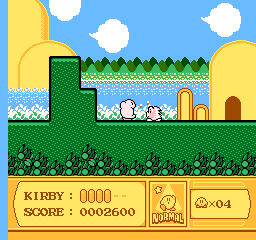
\includegraphics[width=0.5\linewidth]{Kirby.PNG}
	\caption{Kirby's Adventure for NES }
\end{figure}

\begin{figure}[]
	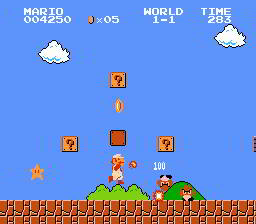
\includegraphics[width=0.5\linewidth]{mario.JPG}
	\caption{Super Mario Bros for NES }
\end{figure}



\section{What is the intended aesthetic?}


\section{Is the scope appropriate for the product development time-frame?}

	
\end{document}